\documentclass{article}
\usepackage[utf8]{inputenc}
\usepackage[spanish]{babel}
\usepackage{listings}
\usepackage{float}
\usepackage{graphicx}
\graphicspath{ {images/} }
\usepackage{cite}

\begin{document}

\begin{titlepage}
    \begin{center}
        \vspace*{1cm}
            
        \Huge
        \textbf{PARCIAL \#1}
            
        \vspace{0.5cm}
        \LARGE
        Informa2 S.A.S.
            
        \vspace{1.5cm}
            
        \textbf{David Santiago Rojo Castrillon}
            
        \vfill
            
        \vspace{0.8cm}
            
        \Large
        Departamento de Ingeniería Electrónica y Telecomunicaciones\\
        Universidad de Antioquia\\
        Medellín\\
        23 de Abril de 2021
            
    \end{center}
\end{titlepage}

\tableofcontents
\newpage
\section{Sección introductoria}\label{intro}
El principal objetivo de esta actividad es poner en práctica los conocimientos aprendidos en informática II y en cursos previos de programación o circuitos eléctricos, se pondrán a prueba las habilidades en cuanto a la resolución de problemas. Es una actividad que además de combinar la programación y el montaje de circuitos con Arduino a la vez permite afrontar problemas del mundo laboral.

\section{Análisis del problema} \label{contenido}
La actividad se basa en la creación de un prototipo de pantalla luminosa la cual se compone de 64 bombillos ledes, estas se han convertido en un objeto frecuente en todo tipo de localidad, sea un restaurante, un anuncio de tránsito, ente otros.
El problema se divide en 2 dos partes, primero será necesario llevar a cabo el montaje del circuito, usando las indicaciones y la documentación suministradas por los maestros; luego de tener el montaje completamente funcional, la siguiente labor es la implementación de código para realizar los diferentes requerimientos.


\section{Tareas definidas} \label{contenido}
\subsection{Investigación}
Para llevar a cabo esta actividad son necesarios algunos conceptos adicionales, ya que usar pocos puertos y conectar varios integrados en conjunto son conceptos desconocidos por ahora, es coherente hacer una investigación en la documentación del integrado y consultar mas sobre los puertos digitales de un Arduino.

Los puertos digitales del Arduino nos permiten manejar perifericos a traves de ellos, pero solo un numero limitado de ellos, tantos como pines disponibles tengamos, pero al momento de necesitar manejar mas de 60 componentes y no tener la posibilidad de usar una cantidad de exagerdad de Arduinos, la principal solución es usar un registro de desplazamiento (74HC595)

\begin{figure}[H]
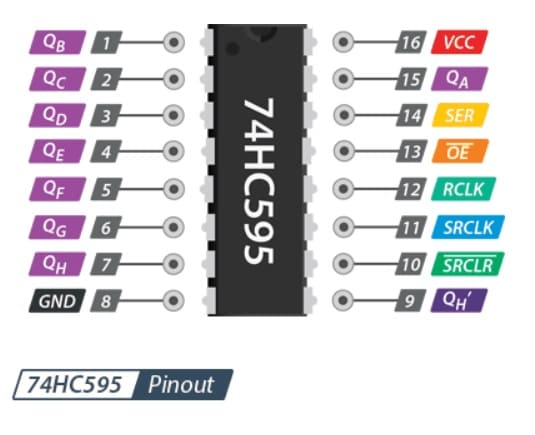
\includegraphics[width=8cm]{pinout-74HC595.jpg}
\centering
\caption{C.I. 74HC595}
\label{fig:chip}
\end{figure}

\subsection{Montaje circuito}
El montaje del circuito es una de las principales tareas a afrontar, se debe hacer el arreglo de 64 ledes, con sus respectivas resistencias (en este caso de 560 Ohm c/u). Para controlar esta cantidad de ledes a través del Arduino haremos uso del circuito integrado 74HC595. En este caso se usará un C.I. por cada fila (en total 8) haciendo uso de tan solo 3 pines digitales del Arduino.

\subsection{Codificacion tareas}
\textbf{FUNCIONES PARA EL MANEJO DEL CHIP:}\par
o	void ledWrite() //Funcion que recibe 8 enteros, para encender 8 filas de ledes\par
o	void patron1 () //Muestrar el patron solicitado en el primer punto (es el \#5)\par
o	void verificacion() //Verificar el funcionamiento de los 64 ledes\par
\textbf{FUNCIONES PARA EL MANEJO DEL ARREGLO DINAMICO:}\\
o	void CreateList() // Crear una nueva lista\\
o	void AddItem(int item) // Añadir elemento al final de la lista\\
o	void RemoveTail() // Eliminar ultimo elemento de la lista\\
o	void Trim() // Reducir capacidad de la lista al numero de elementos\\
o	void resize() // Reescalar lista\\
o	void printList() // Muestra la lista por Serial para debug\\
o	void askData() //Pide los datos para guardarlos en el arreglo\\
o	void askData4() //Pide los datos para guardarlos en el arreglo (P4)\\
\textbf{FUNCIONES CONVENCIONALES:}\\
o	void setup() // Una repetición.\\
o	void loop() //Ciclo infinito\\

\subsection{Codigo Arduino}
%
A continuación se presenta el codigo implementado.

\begin{lstlisting}[language=C++, label=codigo_ejemplo]
//VARIABLES GLOBALES MANEJO DEL CHIP
int opcion = 0;
int SER  = 2;
int RCLK = 3;
int SRCLK = 4;
#define TEMPO 150
////////////////////////////////////////////////////////////
//VARIABLES GOBLALES PARA MANEJO DEL ARREGLO DINAMICO
int aux = 0;
int num = 0; //Cantidad de patrones (P4)
int retardo = 0; //Retardo entre patrones (P4)
int iter = 0; //Iterador (P4)
int* list;
size_t count;
size_t capacity;
#define PAUSE 1500
///////////////////////////////////////////////////////////

//FUNCIONES MANEJO DEL CHIP
void ledWrite(int ALed, int BLed, int CLed, int DLed, int ELed, int FLed, int GLed, int HLed){//Funcion para escribir en la matriz
   shiftOut(SER, SRCLK, LSBFIRST, HLed);
   shiftOut(SER, SRCLK, LSBFIRST, GLed);
   shiftOut(SER, SRCLK, LSBFIRST, FLed);
   shiftOut(SER, SRCLK, LSBFIRST, ELed);
   shiftOut(SER, SRCLK, LSBFIRST, DLed);
   shiftOut(SER, SRCLK, LSBFIRST, CLed);
   shiftOut(SER, SRCLK, LSBFIRST, BLed);
   shiftOut(SER, SRCLK, LSBFIRST, ALed);
   digitalWrite(RCLK, HIGH);
   digitalWrite(RCLK, LOW);
}

void patron1 (){//DE ESTA FORMA SACAMOS EL 5:
  ledWrite(B01111110,255,B11000111,B00000111,B11111110,B11100000,255,255);
  delay(TEMPO); 
}

void verificacion(){//DE ESTA FORMA PRENDEMOS TODOS:
  ledWrite(255,255,255,255,255,255,255,255); delay(TEMPO);  
}

void patron2(){//DIAGONALES INTERCALADAS
//USADA PARA VERIFICACIONES DE FUNCIONAMIENTO
  ledWrite(B10000000,B01000000,B00100000,B00010000,B00001000,B00000100,B00000010,B00000001); delay(TEMPO);
  ledWrite(B00000001,B00000010,B00000100,B00001000,B00010000,B00100000,B01000000,B10000000); delay(TEMPO);
}
///////////////////////////////////////////////////////////////////////////////////////

//FUNCIONES PARA MANEJO DEL ARREGLO DINAMICO
void CreateList(size_t _capacity) {// Crear una nueva lista
  list = new int[_capacity];
  capacity = _capacity;
  count = 0;
}


void AddItem(int item) {// Añadir elemento al final de la lista
  ++count;
    
  if (count > capacity)
  {
    size_t newSize = capacity * 2;
    resize(newSize);
  } 

  list[count - 1] = item;
}


void RemoveTail() {// Eliminar ultimo elemento de la lista
  --count;
}

void Trim() {// Reducir capacidad de la lista al numero de elementos
  resize(count);
}

void resize(size_t newCapacity) {// Reescalar lista
  int* newList = new int[newCapacity];
  memmove(newList, list, count  * sizeof(int));
  delete[] list;
  capacity = newCapacity;
  list = newList;
}

void printList() {// Muestra la lista por Serial para debug
  Serial.print("Capacity:");
  Serial.print(capacity);

  Serial.print("  Count:");
  Serial.print(count);

  Serial.print("  Items:");
  for (size_t index = 0; index < count; index++)
  {
    Serial.print(list[index]);
    Serial.print(' ');
  }
  Serial.println();
}

void askData() {//Pide los datos para guardarlos en el arreglo
	Serial.println("Lista con 8 elementos");
    CreateList(8);
    Serial.println();

    for(int i=0; i<8; i++){
      //Serial.println();
      Serial.print("Introducir la fila #");
      Serial.print(i+1);
      Serial.print(": ");delay(PAUSE);
      aux = Serial.parseInt();
      Serial.println(aux);
      AddItem(aux);
    }  
}

void askData4() {//Pide los datos para guardarlos en el arreglo (P4)
	Serial.println("Cuantos patrones va a ingresar?");delay(PAUSE);
  	num = Serial.parseInt();
  	Serial.println(num);
    CreateList((num*8));
    Serial.println();

    for(int i=0; i<(num*8); i++){
      //Serial.println();
      Serial.print("Introducir la fila #");
      Serial.print(i+1);
      Serial.print(": ");delay(PAUSE);
      aux = Serial.parseInt();
      Serial.println(aux);
      AddItem(aux);
    }  
}
///////////////////////////////////////////////////////////


//FUNCIONES CONVENCIONALES
void setup(){
    //INICIALIZAMOS LOS PUERTOS
   pinMode(SER, OUTPUT);
   pinMode(RCLK, OUTPUT);
   pinMode(SRCLK, OUTPUT);
   Serial.begin(9600);//Inicializar Serial
   int op = 0;
  
  //PREGUNTA SI DESEA AGREGAR UNA MATRIZ (P)
   Serial.println("Desea crear una matriz propia para el punto 3?");
   Serial.println("1. SI ----- 2. NO"); delay(PAUSE);
   op = Serial.parseInt();
   Serial.println(op);
  
   if(op==1){
		askData();
        printList();
   }
  
  //PREGUNTA SI DESEA AGREGAR MÁS DE UNA MATRIZ (P4)
  Serial.println("Desea crear una o mas matrices propias para el punto 4?");
  Serial.println("1. SI ----- 2. NO"); delay(PAUSE);
  op = Serial.parseInt();
  Serial.println(op);
  
  if(op==1){
    Serial.println("Que retardo quiere entre patrones: "); delay(PAUSE);
    retardo = Serial.parseInt();
    Serial.println(retardo);
	askData4();
    printList();
    Serial.println();
    Serial.println(retardo);
    retardo = retardo*1000;
  }
  
   Serial.println();
   Serial.println("1. Patron 1.");
   Serial.println("2. Verificacion.");
   Serial.println("3. Imagen (PARA ESTE PUNTO MIRAR EL MANUAL...).");
   Serial.println("4. Publik (PARA ESTE PUNTO MIRAR EL MANUAL...).");
   Serial.println("Seleccione una opcion: ");
}

void loop(){
  
    //Condicion que pregunta si hay datos
    if(Serial.available()>0){
   
      opcion = Serial.parseInt(); //Leer como int
      
      Serial.print("opcion seleccionada: ");
      Serial.print(opcion);
   }
  switch(opcion){
    
  case 1:
    Serial.println("Prueba 1");
    patron1();
    break;
    
  case 2:
    Serial.println("Prueba 2");
    verificacion();
    break;
    
  case 3:
    //ledWrite(list[0],list[1],list[2],list[3],list[4],list[5],list[6],list[7]); delay(TEMPO);
    ledWrite(list[iter],list[(iter+1)],list[(iter+2)],list[(iter+3)],list[(iter+4)],list[(iter+5)],list[(iter+6)],list[(iter+7)]); delay(TEMPO);
  	Serial.println("Prueba 3");
 	break;
    
  case 4:
  	Serial.println("Prueba 4");
    for(int i=0; i<(num*8); i+=8){
      ledWrite(list[iter],list[(iter+1)],list[(iter+2)],list[(iter+3)],list[(iter+4)],list[(iter+5)],list[(iter+6)],list[(iter+7)]); delay(TEMPO);
      iter+=8;
      delay(retardo);    
    }
  	break;
  }
}
\end{lstlisting}



\section{Problemas presentados} \label{contenido}
o	\textbf{Con la conexiones:} El primer problema que se presentó con la implementación fue al intentar hacer el montaje de todos los circuitos integrados en una protoboard, por la cantidad de chips empleados (8) era imposible hacer uso de una sola placa, por lo cual eran necesarias dos o más; así comenzó el diseño implementado en placas de prueba (y con los bombillos al aire <<como se le conoce ordinariamente>>) pero esta implementación no pudo ser llevada a cabo por completo, ya que al momento de avanzar del tercer integrado se encontraba pequeños problemas derivados de la conexión, debido a esto fue necesario hacer uso de conexiones al aire (todas directamente a los objetos (circuitos integrados, resistencias, ledes, etc).\par
\begin{figure}[H]
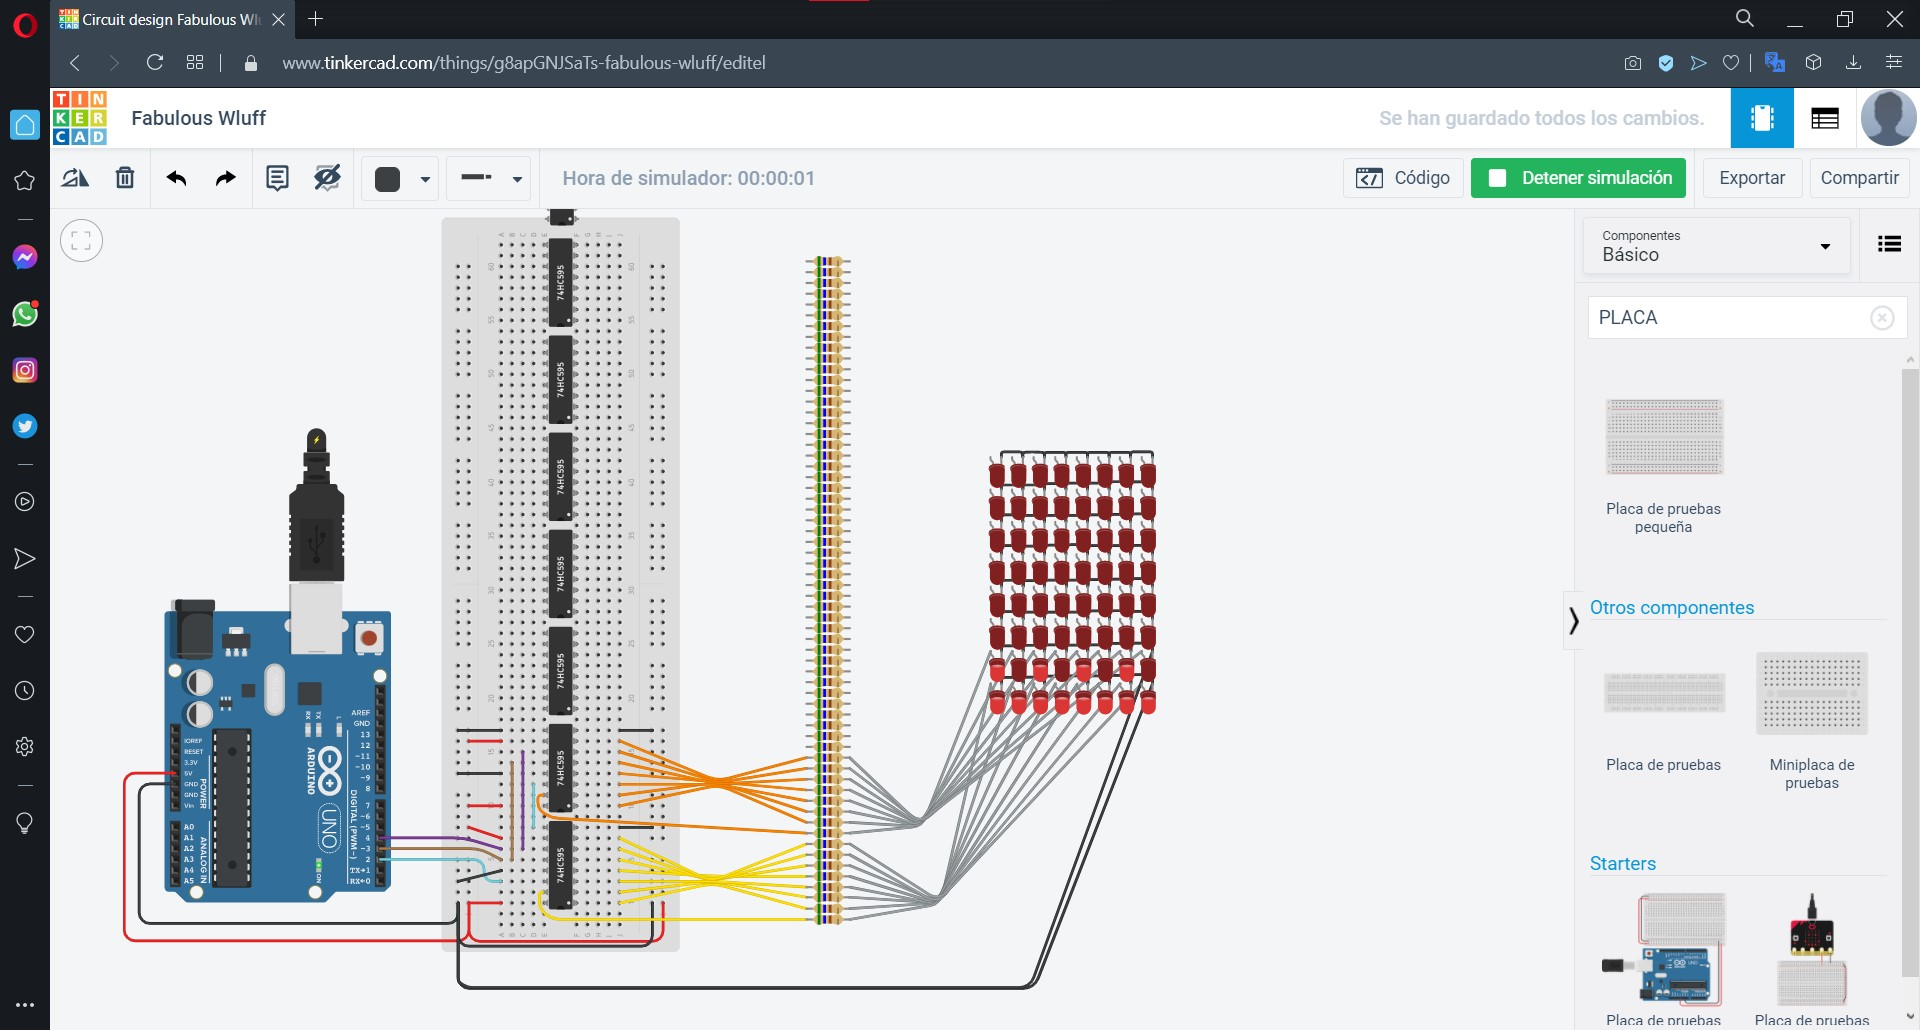
\includegraphics[width=12cm]{protoboard.jpg}
\centering
\caption{Problemas conexiones}
\label{fig:protoboard}
\end{figure}

o	\textbf{Control de versiones:} A medida que el proyecto iba avanzando y que se tenían diferentes conexiones montadas y otras aun en desarrollo, se presenta la necesidad de tener un control de versiones, de poder estar volviendo a un punto estable donde el programa funcionaba según lo esperado, debido a que Tinkercad no cuenta con este sistema, ni tampoco es posible hacerle seguimiento al montaje a través de Github, nace la necesidad de hacer un uso improvisado de control de versiones, haciendo una copia del circuito cada vez que tenemos un punto estable y así en caso de presentar errores más adelante poder volver a retomar desde la copia. (Se adjunta imagen correspondiente)\par
\begin{figure}[H]
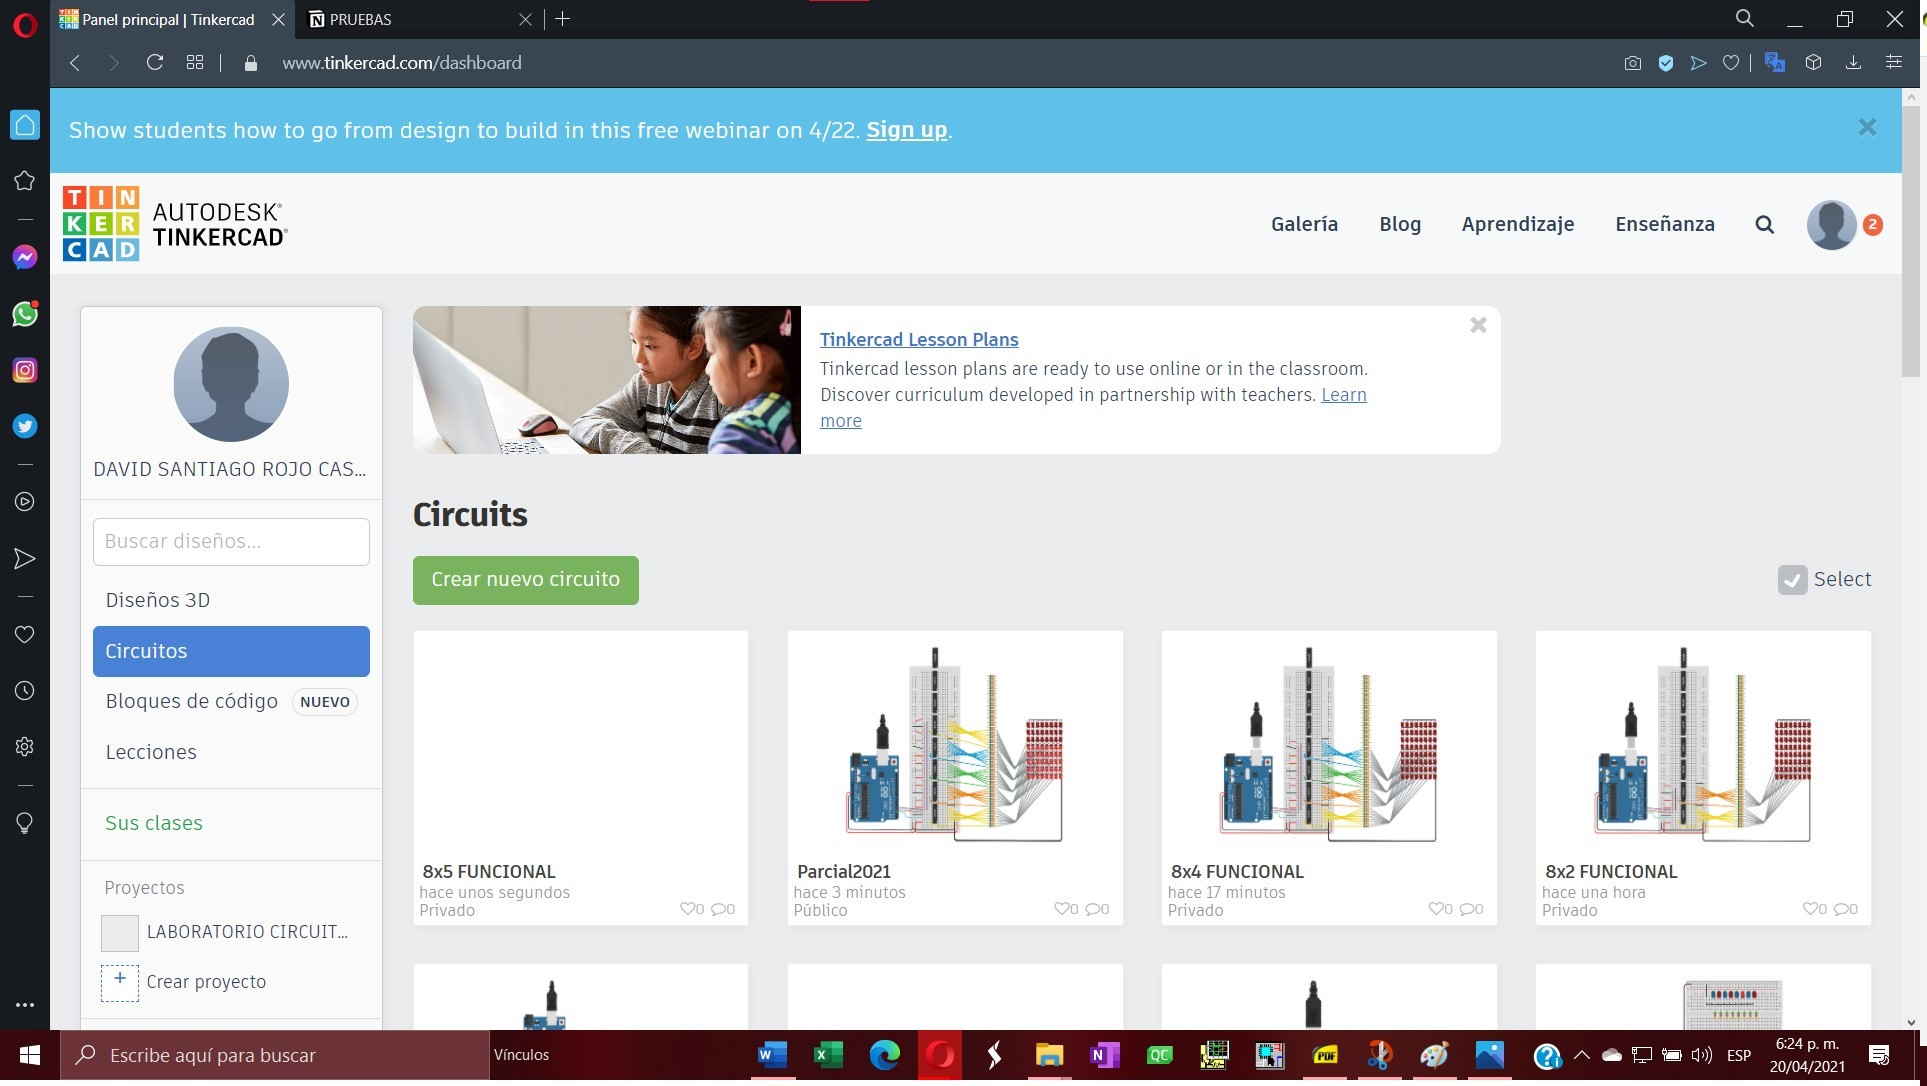
\includegraphics[width=12cm]{control de versiones.jpg}
\centering
\caption{Control de versiones}
\label{fig:control-de-versiones}
\end{figure}

o	\textbf{Tinkercad:} Otro problema que se presentó es debido al alto consumo que requiere la interfaz de Tinkercad, por momentos puede llegar a generar retrasos o congelarse un poco, debemos disponer de un buen equipo y una buena conexión a internet para tener un desarrollo tranquilo de nuestra labor.\par

\section{Consideraciones} \label{contenido}
o	Es muy importante antes de afrontar el problema, investigar sobre los elementos que van a ser usados en la implementación, ya que algunas veces las clases debido al sistema virtual no pueden abarcar o responder todas las inquietudes generadas, es importante conocer bien todos los componentes, para que no se presenten complicaciones durante la implementación.\par
o	Para llevar un desarrollo ordenado y evitar errores, es recomendable hacer uso de todo lo aprendido en las clases teóricas y en los laboratorios, llevar un desarrollo secuencial de funciones, ir desarrollando pequeñas tareas e ir comprobando su funcionamiento, para finalmente hacer el acople de todas las funciones empleadas, en este caso fueron divididas en tres segmentos, funciones para el manejo del chip, funciones para el manejo de arreglos dinámicos y las ya conocidas funciones convencionales de Arduino.\par
o	Finalmente, una consideración mas relacionada con el trabajo en general que con la implementación, es que este tipo de actividades ayudan al estudiante a tener que usar un poco de todo lo aprendido, recapitular bastantes ideas, indagar sobre temas que no quedaron claros, entre otras muchas practicas que conllevan a un mayor aprendizaje.\par

\begin{figure}[H]
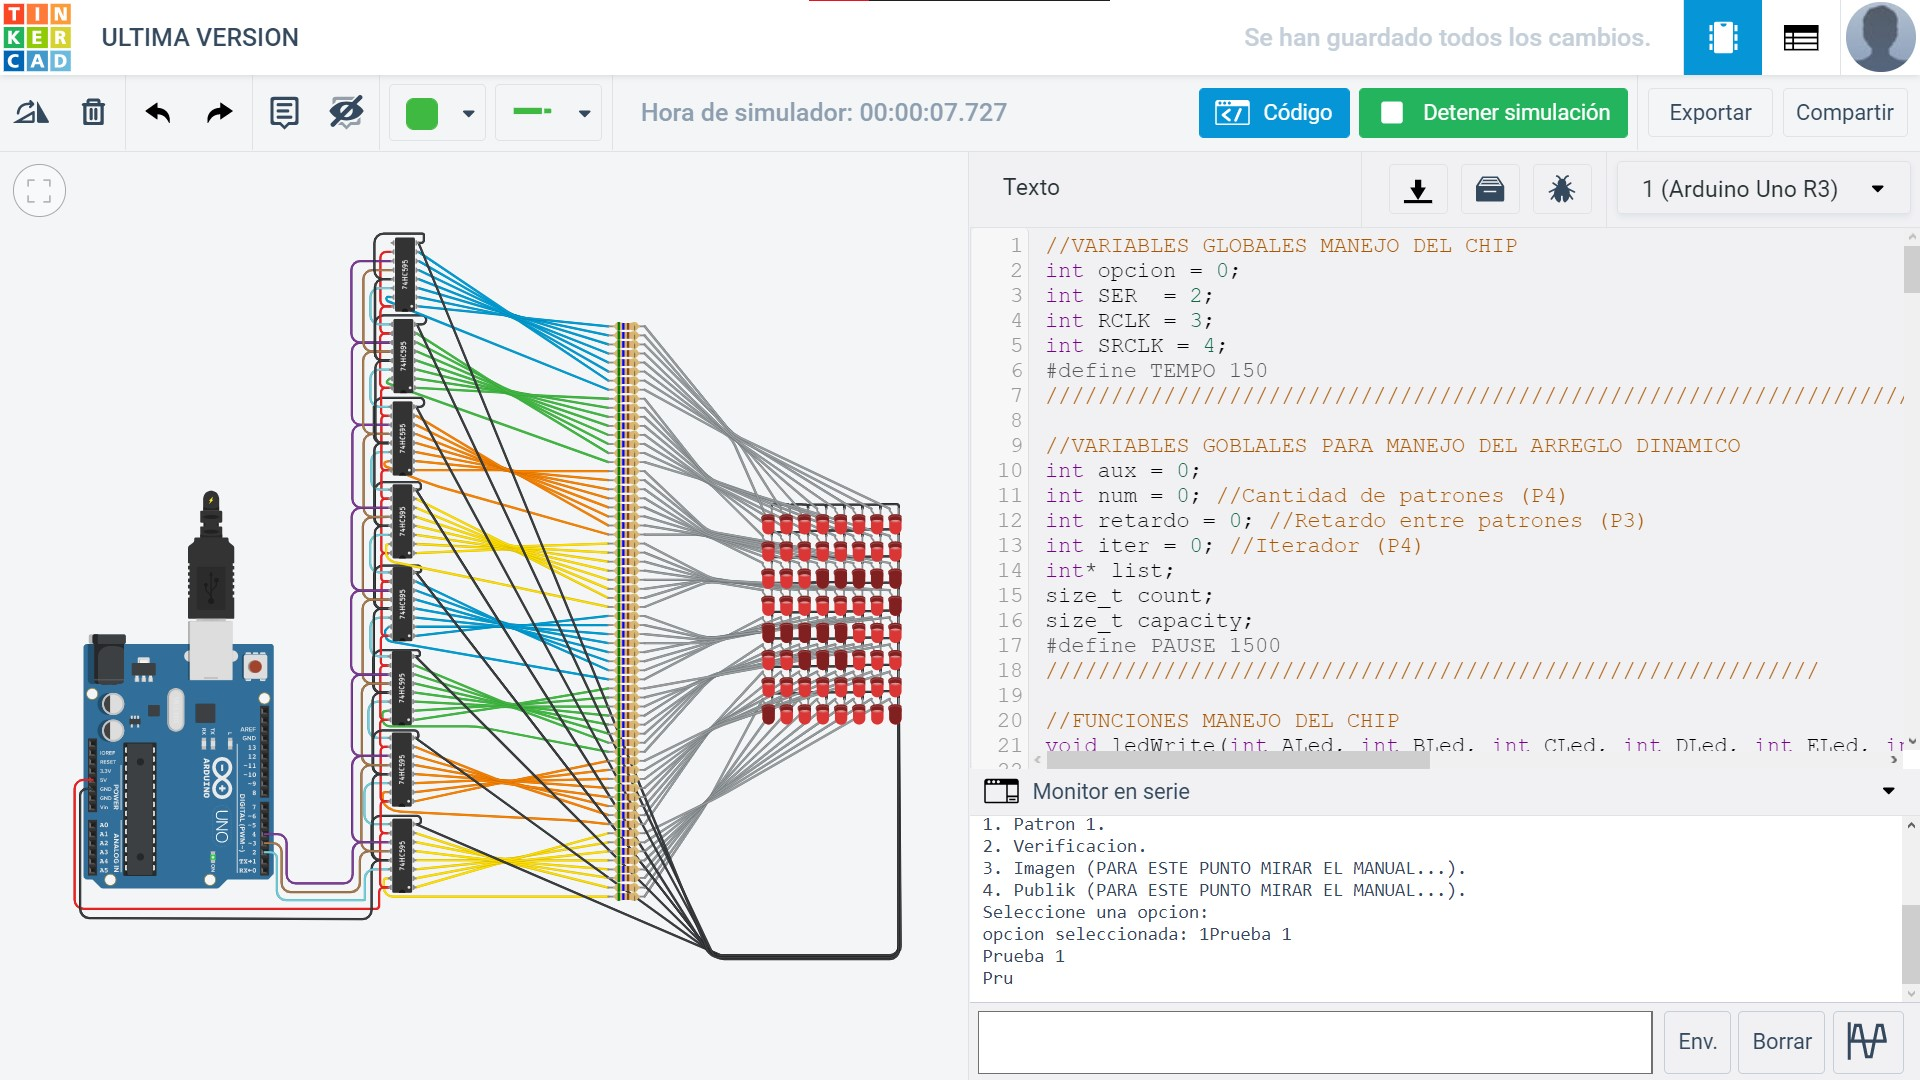
\includegraphics[width=12cm]{Montaje finalizado.jpg}
\centering
\caption{Conexión correcta}
\label{fig:conexion}
\end{figure}

\end{document}
